\documentclass{article}

\usepackage{fancyhdr}
\usepackage{extramarks}
\usepackage{amsmath}
\usepackage{amsthm}
\usepackage{amsfonts}
\usepackage{tikz}
\usepackage[plain]{algorithm}
\usepackage{algpseudocode}
\usepackage{graphicx}
\usepackage{caption}
\usepackage{subcaption}
\usepackage{float}
\usetikzlibrary{automata,positioning}
\usepackage{listings}
%
% Basic Document Settings
%

\topmargin=-0.45in
\evensidemargin=0in
\oddsidemargin=0in
\textwidth=6.5in
\textheight=9.0in
\headsep=0.25in

\linespread{1.1}

\pagestyle{fancy}
\lhead{\hmwkAuthorName}
\chead{\hmwkClass\ (\hmwkClassInstructor\ \hmwkClassTime): \hmwkTitle}
\rhead{\firstxmark}
\lfoot{\lastxmark}
\cfoot{\thepage}

\renewcommand\headrulewidth{0.4pt}
\renewcommand\footrulewidth{0.4pt}

\setlength\parindent{0pt}

%
% Create Problem Sections
%

\newcommand{\enterProblemHeader}[1]{
    \nobreak\extramarks{}{Problem \arabic{#1} continued on next page\ldots}\nobreak{}
    \nobreak\extramarks{Problem \arabic{#1} (continued)}{Problem \arabic{#1} continued on next page\ldots}\nobreak{}
}

\newcommand{\exitProblemHeader}[1]{
    \nobreak\extramarks{Problem \arabic{#1} (continued)}{Problem \arabic{#1} continued on next page\ldots}\nobreak{}
    \stepcounter{#1}
    \nobreak\extramarks{Problem \arabic{#1}}{}\nobreak{}
}

\setcounter{secnumdepth}{0}
\newcounter{partCounter}
\newcounter{homeworkProblemCounter}
\setcounter{homeworkProblemCounter}{1}
\nobreak\extramarks{Problem \arabic{homeworkProblemCounter}}{}\nobreak{}

%
% Homework Problem Environment
%
% This environment takes an optional argument. When given, it will adjust the
% problem counter. This is useful for when the problems given for your
% assignment aren't sequential. See the last 3 problems of this template for an
% example.
%
\newenvironment{homeworkProblem}[1][-1]{
    \ifnum#1>0
        \setcounter{homeworkProblemCounter}{#1}
    \fi
    \section{Problem \arabic{homeworkProblemCounter}}
    \setcounter{partCounter}{1}
    \enterProblemHeader{homeworkProblemCounter}
}{
    \exitProblemHeader{homeworkProblemCounter}
}

%
% Homework Details
%   - Title
%   - Due date
%   - Class
%   - Section/Time
%   - Instructor
%   - Author
%

\newcommand{\hmwkTitle}{Homework\ \#1}
\newcommand{\hmwkDueDate}{September 26, 2014}
\newcommand{\hmwkClass}{STAT5444}
\newcommand{\hmwkClassTime}{12:20 MWF}
\newcommand{\hmwkClassInstructor}{Professor Scott Leman}
\newcommand{\hmwkAuthorName}{Kevin Malhotra}

%
% Title Page
%

\title{
    \vspace{2in}
    \textmd{\textbf{\hmwkClass:\ \hmwkTitle}}\\
    \normalsize\vspace{0.1in}\small{Due\ on\ \hmwkDueDate\ at 3:10pm}\\
    \vspace{0.1in}\large{\textit{\hmwkClassInstructor\ \hmwkClassTime}}
    \vspace{3in}
}

\author{\textbf{\hmwkAuthorName}}
\date{}

\renewcommand{\part}[1]{\textbf{\large Part \Alph{partCounter}}\stepcounter{partCounter}\\}

%
% Various Helper Commands
%

% Useful for algorithms
\newcommand{\alg}[1]{\textsc{\bfseries \footnotesize #1}}

% For derivatives
\newcommand{\deriv}[1]{\frac{\mathrm{d}}{\mathrm{d}x} (#1)}

% For partial derivatives
\newcommand{\pderiv}[2]{\frac{\partial}{\partial #1} (#2)}

% Integral dx
\newcommand{\dx}{\mathrm{d}x}

% Alias for the Solution section header
\newcommand{\solution}{\textbf{\large Solution}}

% Probability commands: Expectation, Variance, Covariance, Bias
\newcommand{\E}{\mathrm{E}}
\newcommand{\Var}{\mathrm{Var}}
\newcommand{\Cov}{\mathrm{Cov}}
\newcommand{\Bias}{\mathrm{Bias}}

\begin{document}

\maketitle

\pagebreak

\begin{homeworkProblem}
\(x_i\) $\mathtt{\sim}$ \(N(\mu, \sigma^2)\) for i = 1, ..., N Assuming \(\sigma^2\) is a known parameter. \\ \\
\( p(\mu|X) \) where \(X = \{x_1, ..., x_N\}\) \\ \\
Part 1: \\
\( L(\mu|X) 
= \prod_{i=1}^{N} \frac {1}{\sqrt{2\pi}\sigma} e^{\frac{-1}{2}\frac{(x_i - \mu)}{\sigma^2}}\) \\ \\
Part 2: \\
\(p(\mu) \propto 1\) \\ \\
\(p(\mu|X) = L(\mu|X)p(\mu) \) \\ \\
\( = \prod_{i=1}^{N} \frac {1}{\sqrt{2\pi}\sigma} e^{\frac{-1}{2}\frac{(x_i - \mu)}{\sigma^2}} * 1\) \\ \\
\( \propto e^{\frac{-1}{2}\frac{\sum_{i=1}^{N}(x_i -\mu)}{\sigma^2}} \) \\ \\
\( = e^{\frac{-1}{2}\frac{\sum_{i=1}^{N}(x_i^2 -2x_i\mu + \mu^2)}{\sigma^2}} \) \\ \\
\( \propto e^{\frac{-1}{2}\frac{(-2\sum_{i=1}^{N}x_i\mu +N\mu^2)}{\sigma^2}} \) \\ \\
\( = e^{\frac{-1}{2}\frac{(-2\sum_{i=1}^{N}x_i\mu +N\mu^2)}{\sigma^2}\frac{\frac{1}{N}}{\frac{1}{N}}}\) \\ \\
\( = e^{\frac{-1}{2}\frac{(-2\mu\bar{x} + \mu^2)}{\frac{\sigma^2}{N}}} \) \\ \\
\( = e^{\frac{-1}{2}(\mu^2[\frac{N}{\sigma^2}] -2\mu[\frac{N\bar{x}}{\sigma^2}])} \) \\ \\
Answers: \\ \\
\( p(\mu|X) = e^{\frac{-1}{2}(\mu^2[\frac{N}{\sigma^2}] -2\mu[\frac{N\bar{x}}{\sigma^2}])} \) \\ \\
\(Var(\mu|X) = [\frac{N}{\sigma^2}]^{-1} = \frac{\sigma^2}{N} \) \\ \\ 
\(E(\mu|X) = \frac{N\bar{x}}{\sigma^2}*[\frac{N}{\sigma^2}]^{-1} = \bar{x} \) \\ \\

\end{homeworkProblem}
\pagebreak
\begin{homeworkProblem}
\(X\) $\mathtt{\sim}$ \(Bin(N, p) \) so that \( p(X=x) = ( \begin{array}{c}N\\x\end{array})p^x(1-p)^{N-x} \) \\ \\
Reference prior: \(p\) $\mathtt{\sim}$ \(Beta(\frac{1}{2}, \frac{1}{2}) \)  \\ \\
pdf for \(z\) $\mathtt{\sim}$ \(Beta(\alpha, \beta)\) \\ \\
\(p(x) = \frac{1}{B(\alpha, \beta)}x^{\alpha-1}(1-x)^{\beta-1}\) \\ \\
\(B(\alpha, \beta) = \int_{0}^{1}z^{\alpha-1}(1-z)^{\beta-1}\) \\ \\
Posterior distribution will be a beta distribution. \\ \\
\(p(p|X) \propto L(p|X)p(p) \) \\ \\
\(\propto [( \begin{array}{c}N\\x\end{array})p^x(1-p)^{N-x}] *
 \frac{1}{B(\alpha, \beta)}p^{\alpha-1}(1-p)^{\beta-1} \) \\ \\
\(\propto [p^x(1-p)^{N-x}] * p^{\alpha-1}(1-p)^{\beta-1} \) \\ \\
\(= p^{x + \alpha - 1} (1-p)^{N-x + \beta -1} \) \\ \\
\(= p^{\alpha^{*}- 1} (1-p)^{\beta^{*} -1} \) \\ \\
\(\alpha^{*} = x + \alpha \rightarrow \alpha^{*} = x + \frac{1}{2} \) \\ \\
\(\beta^{*} = N - x + \beta \rightarrow \beta^{*} = N - x + \frac{1}{2}\) \\ \\
Answers: \\ \\
\(p(p|X) \propto p^{\alpha^{*}- 1} (1-p)^{\beta^{*} -1} \) \\ \\
\(\alpha^{*} = x + \alpha \rightarrow \alpha^{*} = x + \frac{1}{2} \) \\ \\
\(\beta^{*} = N - x + \beta \rightarrow \beta^{*} = N - x + \frac{1}{2}\) \\ \\
If samples are I.I.D then the posterior parameters are: \\ 
\(\alpha^{*} = \sum_{i=1}^Z x + \alpha \rightarrow \alpha^{*} =\sum_{i=1}^Z x x + \frac{1}{2} \) \\ \\
\(\beta^{*} = N - \sum_{i=1}^Z x + \beta \rightarrow \beta^{*} = N - \sum_{i=1}^Z x x + \frac{1}{2}\) \\ \\
\end{homeworkProblem}
\pagebreak
\begin{homeworkProblem}
\(E[Y] = E[XB + \epsilon] = XB\) since \(\epsilon\) has a expected value of zero \\ \\
\(p(\beta|Y, X) = L(\beta|Y, X)*P(\beta) \) \\ \\
\(= e^{\frac{-1}{2}(Y-XB)^T\Sigma^{-1}(Y-XB)} \) \\ \\
\(=e^{\frac{-1}{2}(Y-XB)^T(\sigma^2I)^{-1}(Y-XB)} \) \\ \\
\(=e^{\frac{-1}{2\sigma^2}(Y-XB)^T(Y-XB)} \) \\ \\
\(=e^{\frac{-1}{2\sigma^2}(Y^T - B^TX^T)(Y-XB)} \) \\ \\
\(=e^{\frac{-1}{2\sigma^2}(Y^TY -)(Y-XB)} \) \\ \\
\(=e^{\frac{-1}{2\sigma^2}(Y^TY - B^TX^TY - Y^TXB + B^TX^TXB)} \) \\ \\
\(\propto e^{\frac{-1}{2\sigma^2}(-2B^TX^TY + B^TX^TXB)} \) \\ \\
\( Var(\beta|X, Y) = \sigma^2 (X^TX)^{-1} \) \\ \\
\( E(\beta|X, Y) = \sigma^2 (X^TX)^{-1} * \frac{X^TY}{\sigma^2} = (X^TX)^{-1}X^TY\) \\ \\
Answers: \\ \\
\(p(\beta|Y,X) \propto e^{\frac{-1}{2\sigma^2}(-2B^TX^TY + B^TX^TXB)} \) \\ \\
\( Var(\beta|X, Y) = \sigma^2 (X^TX)^{-1} \) \\ \\
\( E(\beta|X, Y) = \sigma^2 (X^TX)^{-1} * \frac{X^TY}{\sigma^2} = (X^TX)^{-1}X^TY\) \\ \\
Part 2: \\ \\
\(\hat{\beta} =(X^TX)^{-1}X^TY\) \\ \\
\(Var(\hat{\beta}) = Var((X^TX)^{-1}X^TY) \) \\ \\
\(Var(\hat{\beta}) = [(X^TX)^{-1}X^T] * Var(Y) *[ (X^TX)^{-1}X^T]^T \) \\ \\
\(Var(\hat{\beta}) = [(X^TX)^{-1}X^T] * Var(Y) *[ X(X^TX)^{-1}] \) \\ \\
\(Var(\hat{\beta}) = [(X^TX)^{-1}X^T] \Sigma[X(X^TX)^{-1}] \) \\ \\
\(Var(\hat{\beta}) = [(X^TX)^{-1}X^T] \sigma^2 I[X(X^TX)^{-1}] \) \\ \\
\(Var(\hat{\beta}) = \sigma^2[(X^TX)^{-1}X^TX(X^TX)^{-1}] \) \\ \\
\(Var(\hat{\beta}) = \sigma^2(X^TX)^{-1} \) \\ \\
\(E(\hat{\beta}) = (X^TX)^{-1}X^TE(Y) = (X^TX)^{-1}X^TXB = B \) \\ \\
Answers: \\ \\
\(Var(\hat{\beta}) = \sigma^2(X^TX)^{-1} \) \\ \\
\(E(\hat{\beta}) = B \) \\ \\
The variances are the same, but the expected values are different. The Posterior distribution's expected value is equivalent to \( \hat{\beta} \). This makes sense since the MLE will approach \( \beta \). In conclusion, they both vary equivalent just centered around the ground truth \(\beta\) or the posterior truth \( \hat{\beta} \).
\end{homeworkProblem}
\begin{homeworkProblem}
Blood Type in 0.01 of population is innocent. \(P(E|I) = 0.01\) \\ \\
Blood is found with no innocent explanation. \(P(E| \char `\~ I) = 1\) \\ \\
\(P(E|I) = 0.01 = P(I|E)\) (Fallacy) \\ \\
\(P(\char `\~ I|E) = 1-P(I|E) = 0.99 \)\\ \\
\(P(\char `\~ I|E) = \frac{P(E|\char `\~ I)P(\char `\~ I)}
{P(E|\char `\~ I)P(\char `\~ I) + P(E|I)P(I)} = 0.99 \)\\ \\
\(P(\char `\~ I|E) = \frac{1*(1- P(I))}{1*(1- P(I)) + P(E|I)P(I)} = 0.99\)\\ \\
\(P(\char `\~ I|E) = \frac{(1- P(I))}{(1- P(I)) + 0.01P(I)} = 0.99\)\\ \\
\(P(\char `\~ I|E) = \frac{1- P(I)}{1- 0.99P(I)} = 0.99\)\\ \\
\(P(\char `\~ I|E) = \frac{1- P(I)}{1- 0.99P(I)} = 0.99\)\\ \\
\(P(\char `\~ I|E) = 1- P(I)= 0.99 -0.9801*P(I)\)\\ \\
\(0.01= 0.0199*P(I)\rightarrow P(I) = 0.5025\)\\ \\
Answer: \\ \\
\(P(I) = 0.5025\)\\ \\
The answer is slightly over 0.5, thus his claim is incorrect.
\end{homeworkProblem}
\pagebreak
\begin{homeworkProblem}
\( \Lambda = log(\frac{p}{1-p}) \rightarrow e^\Lambda = \frac{p}{1-p} 
\rightarrow e^\Lambda - e^\Lambda *p = p \rightarrow e^\Lambda = p(1+e^\Lambda) \rightarrow
p = \frac{e^\Lambda}{(1+e^\Lambda)} \) \\ \\
\( g(p)  = \Lambda = log(\frac{p}{1-p}) \) and
\( g^{-1}(\Lambda) = p =\frac{e^\Lambda}{(1+e^\Lambda)} \) \\ \\
Part 1: \\ \\
\(P_p(p) \propto 1 \) \\ \\
\(P_\Lambda(\Lambda) = P_p(g^-1(\Lambda))\mid\frac{d}{d\Lambda}g^-1(\Lambda)\mid \) \\ \\
\(P_\Lambda(\Lambda) = 1* \mid\frac{d}{d\Lambda}\frac{e^\Lambda}{1+e^\Lambda}\mid \) \\ \\
\(P_\Lambda(\Lambda) = 
1* \mid\frac{(1+e^\Lambda)e^\Lambda - e^{2\Lambda}}{(e^\Lambda + 1)^2}\mid \) \\ \\
\(P_\Lambda(\Lambda) = 
1* \mid\frac{e^\Lambda + e^{2\Lambda} - e^{2\Lambda}}{(e^\Lambda + 1)^2}\mid \) \\ \\
\(P_\Lambda(\Lambda) = \mid\frac{e^\Lambda}{(e^\Lambda + 1)^2}\mid \) \\ \\
Answer: \\ \\
\(P_\Lambda(\Lambda) = \frac{e^\Lambda}{(e^\Lambda + 1)^2} \) \\ \\
Part 2: \\ \\
\( P_\Lambda(\Lambda) \propto 1 \) \\ \\ 
\(P_p(p) = P_\Lambda(g^-1(p))\mid\frac{d}{dp}g^-1(p)\mid \) \\ \\
\(P_p(p) = 1 * \mid\frac{d}{dp}log(\frac{p}{1-p})\mid \) \\ \\
\(P_p(p) = \mid\frac{1-p}{p}\frac{d}{dp}\frac{p}{1-p}\mid \) \\ \\
\(P_p(p) = \mid\frac{1-p}{p}\frac{(1-p) - (-1)p}{(1-p)^2}\mid \) \\ \\
\(P_p(p) = \mid\frac{1-p}{p}\frac{1}{(1-p)^2}\mid \) \\ \\
\(P_p(p) = \mid\frac{1}{(1-p)p}\mid \) \\ \\
Answer: \\ \\
\(P_p(p) = \frac{1}{(1-p)p} \) \\ \\
What is the implied prior distribution on p?
\end{homeworkProblem}
\pagebreak
\begin{homeworkProblem}
\begin{figure}[H]
        \begin{subfigure}[b]{0.3\textwidth}
                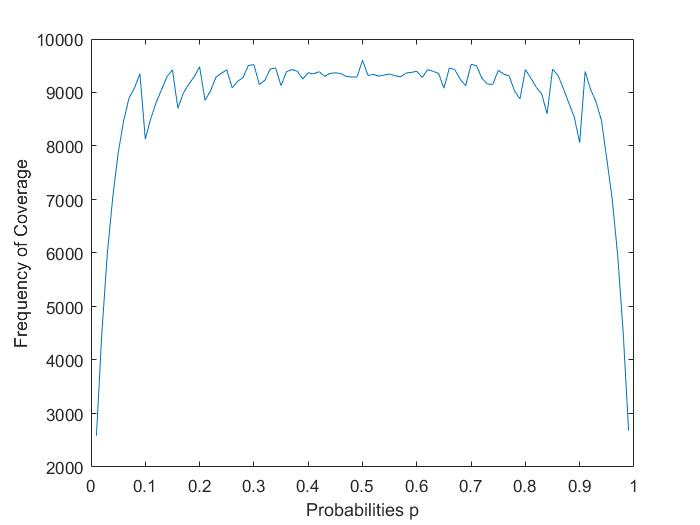
\includegraphics[width=\linewidth]{Problem6N30}
                \caption{N = 30}
                \label{fig:gull2}
        \end{subfigure}%
        \begin{subfigure}[b]{0.3\textwidth}
                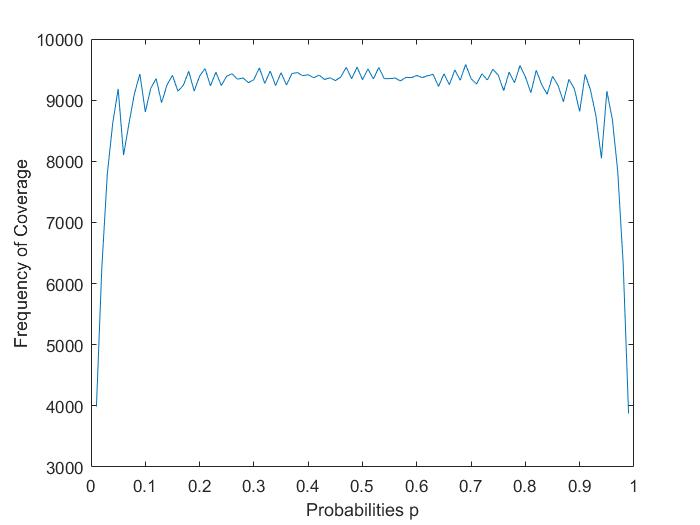
\includegraphics[width=\linewidth]{Problem6N50}
                \caption{N = 50}
                \label{fig:gull2}
        \end{subfigure}%
        \begin{subfigure}[b]{0.3\textwidth}
                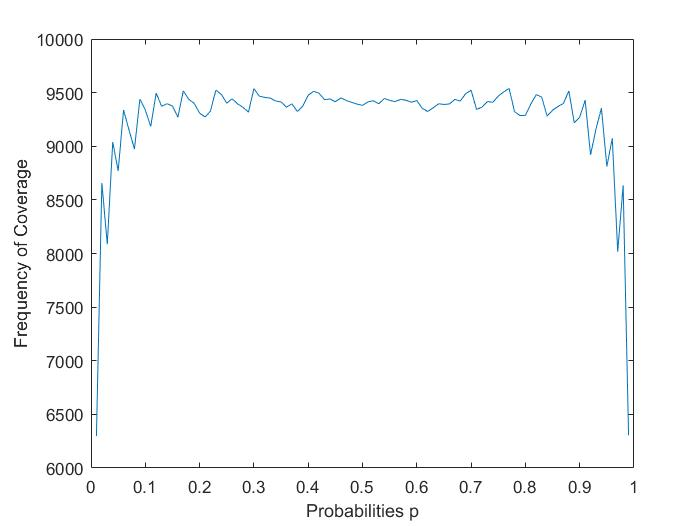
\includegraphics[width=\linewidth]{Problem6N100}
                \caption{N = 100}
                \label{fig:gull2}
        \end{subfigure}%
        \caption{Confidence Interval Coverage}
\end{figure}
Conclude with your thoughts on the experiment. Are you surprised? \\ 
As the number of trials increases the coverage is hitting 95 percent asymptotically. This may be due to the
discrete nature of the draws. Towards the end of the probability spectrum [0, 1] there are a lot less frequencies of hitting the 95 percent coverage section. It seems much more difficult to acquire higher coverage on those sections. \\ \\
Matlab code:
\lstinputlisting{problem6.m}
\end{homeworkProblem}
\end{document}
